\documentclass{article}
\usepackage[
        a4paper,% other options: a3paper, a5paper, etc
        left=3cm,
        right=3cm,
        top=3cm,
        bottom=4cm,
        % use vmargin=2cm to make vertical margins equal to 2cm.
        % us  hmargin=3cm to make horizontal margins equal to 3cm.
        % use margin=3cm to make all margins  equal to 3cm.
]{geometry}
%\usepackage[utf8x]{inputenc}
\usepackage{graphicx}
\usepackage{caption}
\usepackage{enumerate}
\usepackage{subcaption}
\usepackage[procnames]{listings}
\usepackage{color}
\usepackage{amssymb}
\usepackage{amsmath}
\usepackage{comment}
\usepackage{hyperref}
\usepackage{blindtext}
\usepackage[titletoc,title]{appendix}
\usepackage{float}
\usepackage{fullpage}
\definecolor{codegreen}{rgb}{0,0.6,0}
\definecolor{codegray}{rgb}{0.5,0.5,0.5}
\definecolor{codepurple}{rgb}{0.58,0,0.82}
\definecolor{backcolour}{rgb}{0.95,0.95,0.92}

\lstdefinestyle{mystyle}{
    backgroundcolor=\color{backcolour},
    commentstyle=\color{codegreen},
    keywordstyle=\color{magenta},
    numberstyle=\tiny\color{codegray},
    stringstyle=\color{codepurple},
    basicstyle=\ttfamily,
    breakatwhitespace=false,
    breaklines=true,
    captionpos=t,
    keepspaces=true,
    numbers=left,
    numbersep=5pt,
    showspaces=false,
    showstringspaces=false,
    showtabs=false,
    tabsize=2
}

\lstset{style=mystyle, language=Matlab}

\renewcommand{\thesection}{\large{Exercise \arabic{section}}}

\title{Computer Vision - Lab 3}
\author{Luuk Boulogne (s2366681) \and Steven Bosch (s1861948)}
\date{\today}

\begin{document}
\maketitle

\section{}
We use the imshow function in Matlab to select the pixels of three feature points: (1) the top point of the top right letter on the box below the statue ($P_L = (178,271)$, $P_R = (167,271)$), (2) the right bottom point of the yellow blob on the blue can ($P_L = (212, 88)$, $P_R = (204, 88)$) and (3) the left point of the bottom screw in the lamp ($P_L = (292,156)$, $P_R = (278,156)$). We chose these points, because they are easily identifiable for us to select in both images, and they represent the same 3D locations. This is the reason we did not, for example, take the edge of the lamp or statue, because the edge represents different 3D locations from different angles. 

Calculating the disparity as $u_L - u_R$ gives us the following disparities for the three points: (box) 11, (can) 8 and (lamp) 14. In the ground truth images we find the following gray scale values: (box) 111, (can) 55, (lamp) 190. To see how our approaches compare, we look at the proportions between these points, given in table \ref{table1}

\begin{table}[!ht]
 \centering
 \caption{Proportions between different feature points}
 \begin{tabular}{c|c|c}
 Ratios & Manual feature points & Ground truth \\
 \hline
 $box/can$ & 1.375 & 2.02 \\
 $can/lamp$ & 0.57 & 0.29 \\
 $box/lamp$ & 0.79 & 0.58
 \end{tabular}
 \label{table1}
\end{table}

As we can see from the table, the proportions differ quite significantly. Assuming that the ground truth is completely accurate, our method does not seem very accurate, in contrast to our expectations. We expected the result to be quite accurate, since we take exactly the same locations in 3D and we, as humans, are very good at recognizing similar points in two images. What we lack though, is the capacity to determine exact curvature of edges, which is what a computer of course is capable of. Perhaps that has influenced our manual selection in such a way that we were inaccurate. However, as we explained above, it is probably not best to use edges of 3D objects, since those edges do not always represent the same 3D locations on two images taken from different angles. What a computer also is better in, is to take the average x and y coordinate of a blob (feature). This can be useful, since from different angles the same blob can have different sizes and you would want to take the middle of the blob to be able to compare the two. In this case we, as humans, just had to guess the middle, while a computer can just calculate the average.

\section{}
\section{}
\section{}
To match the images using SIFT-features we first convert the image into grayscale images and then run the script given in appendix \ref{code:SIFT}. In this script we calculate the disparities between the matches that have a maximum difference of two y-pixels and store it together with the coordinates. Furthermore the y-differences and the number of equal y-values and the maximum y-value are stored.

Figure \ref{matches} shows the matches between the two images. As we can observe, the matches are all near-horizontal. However, if we look at the number of equal y-values, this is only 

\begin{figure}
 \centering
 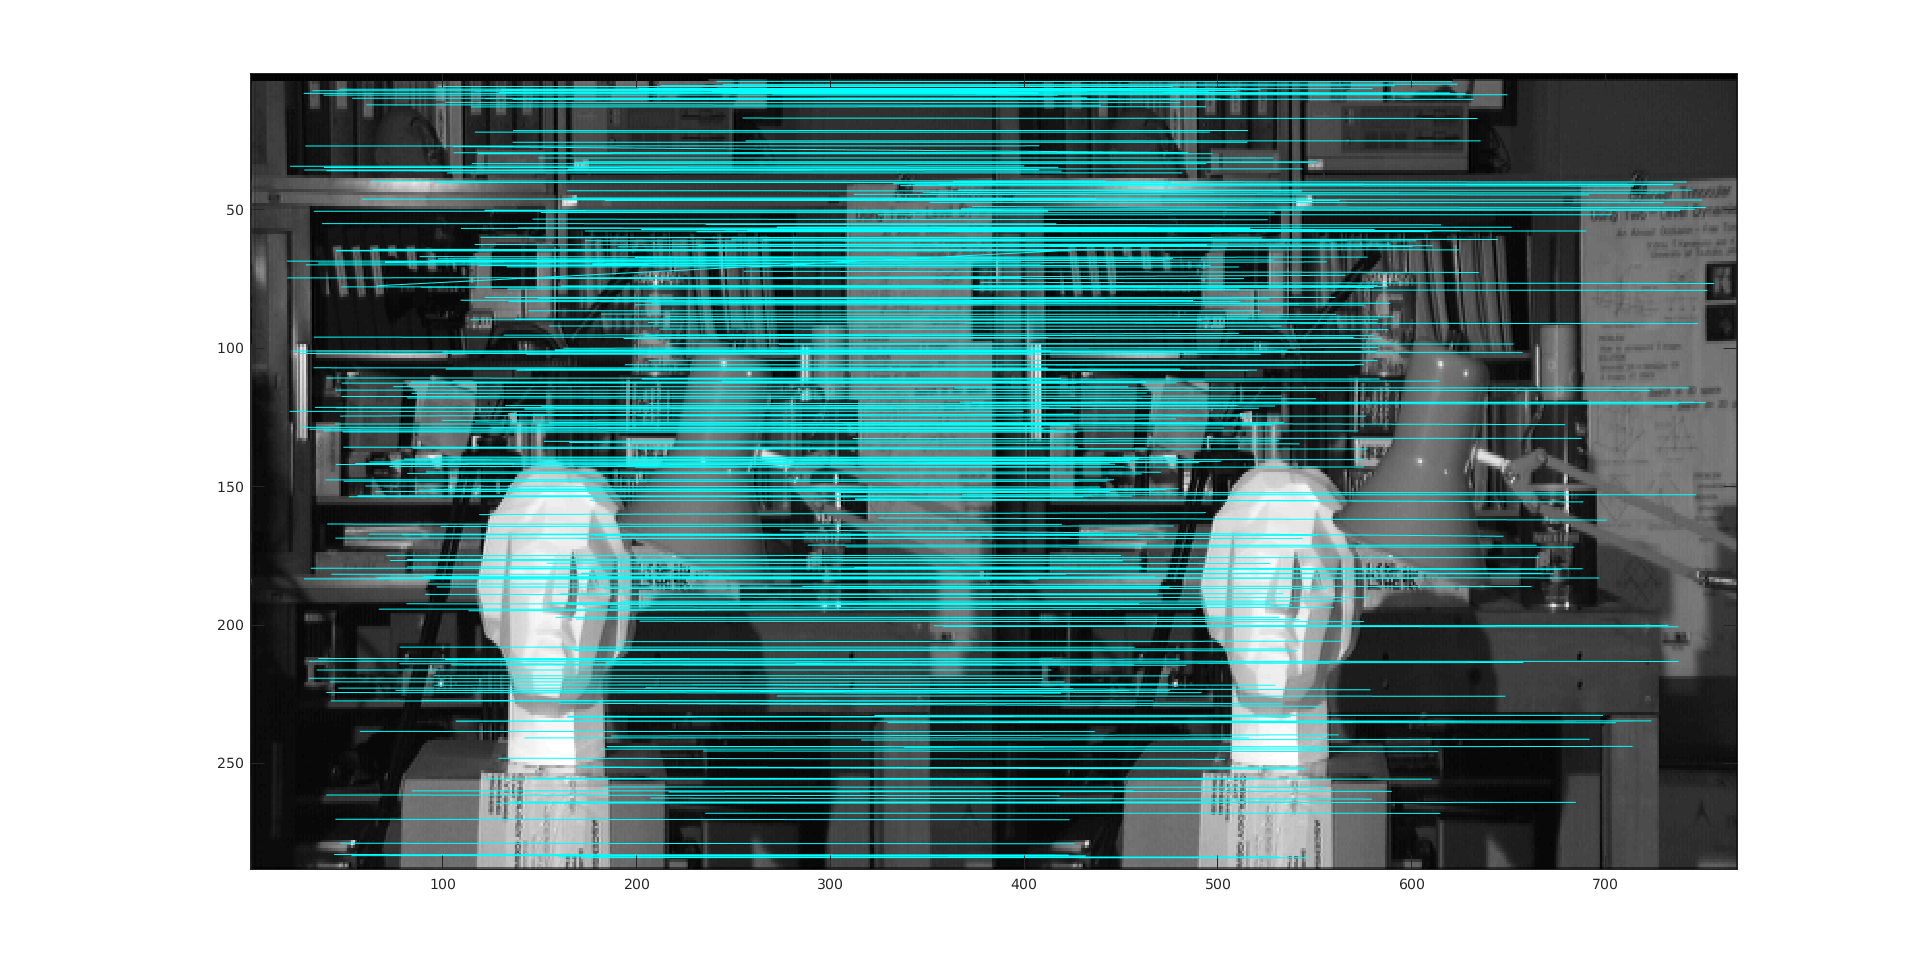
\includegraphics[width = \linewidth]{matches.png}
 \caption{The found matches between the two images by using SIFT features}
 \label{matches}
\end{figure}

\begin{appendices}
\section{Code}
\lstinputlisting[caption={Script to determine the disparities using SIFT-features},label={code:SIFT}]{../SIFT/stereoSift.m}
\end{appendices}

\end{document}